%%%%%%%%%%%%%%%%%%%%%%%%%%%%%%%%%%%%%%%%%%%%%%%%%%%%%%%%%%%%%%%%
\chapter{解集合プログラミングを用いたハミルトン路・閉路問題のASP符号化}
%%%%%%%%%%%%%%%%%%%%%%%%%%%%%%%%%%%%%%%%%%%%%%%%%%%%%%%%%%%%%%%%
本章では,ASPを用いた第\ref{sec:background}章にて説明した諸問題を解く流れと提案する符号化について説明する.
まずは,本研究でASPシステム \clingo を用いて諸問題を解いた流れを図\ref{aspmethod}に図示したので,
これについて解説する.
はじめに2つのファイルを作成した.
図における''問題''にあたるグラフを,ASPシステムが読み取れるように,ASPファクト形式で記述したものと,
諸問題をASP符号化したものである.
これらをASPシステムに処理させることで,解集合が出力される.
この解集合が諸問題の解,つまりは条件を満たしたハミルトン路・閉路を表している.

以下,本章ではASPファクト形式でのグラフの表現と,提案するASP符号化手法について説明する.
\begin{figure}[tbp]
\tikz{
  %1ノード目
  \path[draw=black, fill=blue!20, rounded corners=5pt]%線の設定
  node[at={(0.75,0.75)}] {問題}%文字を入れる
  (0,0) --(1.5,0) --(1.5,1.5) --(0,1.5) --cycle;%外周
  %2ノード目
  \path[draw=black, fill=blue!20, rounded corners=5pt, shift={(3,0)}]
  node[at={(0.75,0.75)}] {
    \begin{tabular}{c}
      ASP\\
      ファクト
    \end{tabular}
  }
  (0,0) --(1.5,0) --(1.5,1.5) --(0,1.5) --cycle;
  %3ノード目文字が複数行
  \path[draw=black, fill=green!20, rounded corners=5pt, shift={(6,0)}]
  node[at={(0.75,0.75)}] {
    \begin{tabular}{c}
      ASP\\
      システム
    \end{tabular}
  }
  (0,0) --(1.5,0) --(1.5,1.5) --(0,1.5) --cycle;
  %4ノード目文字が複数行
  \path[draw=black, fill=blue!20, rounded corners=5pt, shift={(9,0)}]
  node[at={(0.75,0.75)}] {解集合}
  (0,0) --(1.5,0) --(1.5,1.5) --(0,1.5) --cycle;
  %5ノード目文字が複数行
  \path[draw=black, fill=red!20, rounded corners=5pt, shift={(3,-3)}]
  node[at={(0.75,0.75)}] {
    \begin{tabular}{c}
      ASP\\
      符号化
    \end{tabular}
  }
  (0,0) --(1.5,0) --(1.5,1.5) --(0,1.5) --cycle;
  \draw[arrows=->] (1.5,0.75) --(3.0,0.75);
  \draw[arrows=->,shift={(3,0)}] (1.5,0.75) --(3.0,0.75);
  \draw[arrows=->,shift={(6,0)}] (1.5,0.75) --(3.0,0.75);
  \draw[arrows=->] (4.5,-2.25) --(6.0,0.5);
}
\caption{ASPを用いた解法}
\label{aspmethod}
\end{figure}

%%%%%%%%%%%%%%%%%%%%%%%%%%%%%%%%%%%%%%%%%%%%%%%%%%%%%%%%%%%%%%%%%%%%%%%
\section{ASPファクト形式}
%%%%%%%%%%%%%%%%%%%%%%%%%%%%%%
\begin{figure}[tbp]
\begin{center}
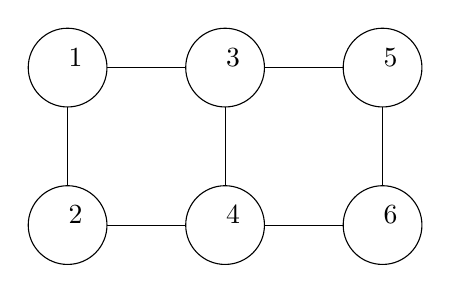
\begin{tikzpicture}
  %ノード1  
  \draw(4,2) circle (0.5)
  node[at={(4.1,2.1)}] {
    \begin{tabular}{c}
      1
    \end{tabular}
  };
  %ノード2  
  \draw(4,0) circle (0.5)
  node[at={(4.1,0.1)}] {
    \begin{tabular}{c}
      2
    \end{tabular}
  };
  %ノード3  
  \draw(6,2) circle (0.5)
  node[at={(6.1,2.1)}] {
    \begin{tabular}{c}
      3
    \end{tabular}
  };
  %ノード4  
  \draw(6,0) circle (0.5)
  node[at={(6.1,0.1)}] {
    \begin{tabular}{c}
      4
    \end{tabular}
  };
  %ノード5  
  \draw(8,2) circle (0.5)
  node[at={(8.1,2.1)}] {
    \begin{tabular}{c}
      5
    \end{tabular}
  };
  %ノード6  
  \draw(8,0) circle (0.5)
  node[at={(8.1,0.1)}] {
    \begin{tabular}{c}
      6
    \end{tabular}
  };
\draw(4,0.5) --(4,1.5);
\draw(6,0.5) --(6,1.5);
\draw(8,0.5) --(8,1.5);
\draw(4.5,0) --(5.5,0);
\draw(4.5,2) --(5.5,2);
\draw(6.5,0) --(7.5,0);
\draw(6.5,2) --(7.5,2);
\end{tikzpicture}

\caption{グラフの例}
\label{graphexample}
\end{center}
\end{figure}
%%%%%%%%%%%%%%%%%%%%%%%%%%%%%%
前述のように,問題をASPシステムに解かせるには,グラフをASPファクト形式にて記述する必要があった.
以下では,図\ref{graphexample}を例として,解説する.
%%%%%%%%%%%%%%%%%%%%%%%%%%%%%%
\lstinputlisting[caption =  図\ref{graphexample}のASPファクト表現,label = graphexamplp]{code/graph_example.lp}
%%%%%%%%%%%%%%%%%%%%%%%%%%%%%%
コード\ref{graphexamplp}は,ASPファクト形式で図\ref{graphexample}のグラフを表現したものである.
アトム\code{node}は各頂点を表し,\code{edge}は各辺を表す.
よって,コード\ref{graphexamplp}の2行目は,頂点が番号1〜6の6つあることを定義し,
5〜7行目では,辺が7つ定義されている.
アトム\code{edge}は2つ引数を持ち,これは表す辺の両端の頂点番号である.
例えば\code{edge(1,2)}は\code{node(1)}と\code{node(2)}を結ぶ無向辺を表す.
最後に,10〜12行目にあるアトム\code{cost}について,図\ref{graphexample}では表記されていないが,これは各辺に割り当てられる重みの値を表す.\code{cost(X,Y,C)}は\code{edge(X,Y}の重みがCであることを定義する.
%%%%%%%%%%%%%%%%%%%%%%%%%%%%%%%%%%%%%%%%%%%%%%%%%%%%%%%%%%%%%%%%%%%%%%%
\section{ハミルトン路・閉路問題のASP符号化}\label{hamiltonianasp}
本研究では,\textbf{undirected},\textbf{directed},\textbf{acyclicity}の3通りのASP符号化を提案する.
これらはいずれもハミルトン路・閉路問題のASP符号化である.

無向グラフ$G=(V,E)$上にハミルトン閉路が存在する必要十分条件は,
以下の2つの制約を満たす部分グラフ$G'=(V,E')$が存在することである.\\
\begin{itemize}
\item $G'$の各頂点の次数が2 \ (次数の制約)\\
\item $G'$が連結である \ (連結の制約)\\
\end{itemize}
本論文では,前者を\textbf{次数の制約},後者を\textbf{連結の制約}と呼ぶ.
ハミルトン閉路問題のASP符号化は,この2つの制約をASP言語のルールで記述することにほとんど等しい.
ただし,ハミルトン路問題では,次数の制約は以下のように変わる.\\
\begin{itemize}
\item ハミルトン路の始点と終点の次数が1,他の頂点の次数が2\\
\end{itemize}

\subsection{undirected}
%%%%%%%%%%%%%%%%%%%%%%%%%%%%%%
\lstinputlisting[caption =  ASP符号化 undirected,label = undirected]{code/hamilton1.lp}
%%%%%%%%%%%%%%%%%%%%%%%%%%%%%%

符号化undirectedはコード\ref{undirected}である.
次数の制約は,3〜8行目に記したように実装し,
連結の制約は,10〜13行目が対応している.
1行目のルールでは,選択子を用いて
「各辺はハミルトン路・閉路に含まれるか,含まれないかのどちらかである」
という制約を実装した.
つまり,アトム\code{in(X,Y)}が解集合に含まれれば,
\code{X}と\code{Y}を両端とする辺が,解となるハミルトン路・閉路に含まれるということである.

次に次数の制約について,ボディに\code{s == t}が含まれる3〜4行目がハミルトン閉路問題に適用されるルールであり,
\code{s != t}が含まれる5〜8行目がハミルトン路問題に適用されるルールである.
なお,変数\code{s}と\code{t}はそれぞれハミルトン路の始点と終点であり,
このように,ハミルトン路問題を解くのか,ハミルトン閉路問題を解くのかの区別にも使われる.
3〜4行目は「各頂点\code{X}について,その次数が2以上2以下である」という制約を,
5〜6行目は「始点\code{s}と終点\code{t}を除く各頂点Xの次数が2以上2以下である」という制約を,
7行目は「始点\code{s}の次数が1以上1以下である」という制約を,
8行目は「終点\code{t}の次数が1以上1以下である」という制約をそれぞれ表している.

続いて,連結の制約については10〜13行目で表現した.
連結の制約は,
「全ての頂点が解となるハミルトン路・閉路を辿ることで始点から到達可能でなければならない」
という制約として実装した.
その実装にあたり,新たに導入したアトム\code{reached(X)}が,
「頂点\code{X}が,解となるハミルトン路・閉路を辿ることで始点\code{s}から到達可能である」という意味を示すように,
10〜12行目のルールを記述した.
まず,始点\code{s}が到達可能でなければならないため,
10行目のファクトを記述した.
11,12行目は,どちらも「頂点\code{X}が到達可能であり,頂点\code{X}と\code{Y}を両端とする辺が解となるハミルトン路・閉路に含まれるならば,頂点\code{Y}も到達可能である.」というルールである.
最後に13行目のルールで「全ての頂点\code{X}が,解となるハミルトン路・閉路を辿ることで始点から到達可能でなければならない」という連結の制約を実装した.
\newpage
符号化directedとacyclicityでは,
与えられた無向グラフを有向グラフ化し,
その有向グラフ上でハミルトン路・閉路を探索する.
\subsection{directed}
%%%%%%%%%%%%%%%%%%%%%%%%%%%%%%
\lstinputlisting[caption =  ASP符号化 directed,label = directed]{code/hamilton2.lp}
%%%%%%%%%%%%%%%%%%%%%%%%%%%%%%
無向グラフ$G$を有向グラフ$G'$として扱うには,
$G$上の全ての無向辺\code{edge(X,Y)}について
有向辺\code{edge(X,Y)},\code{edge(Y,X)}を用意すれば良い.
そのため,コード\ref{directed}の1行目のルールで与えられた無向グラフの有向グラフ化を行った.
2行目は,符号化undirectedと同様,
「各辺はハミルトン路・閉路に含まれるか,含まれないかのどちらかである」
というルールである.

次に次数の制約についてだが,有向グラフ上での次数の制約は無向グラフ上のものとはやや異なる.
ハミルトン路・閉路問題における次数の制約は,有向グラフ$G'$上で,それぞれ以下のようになる.
\begin{itemize}
\item $G'$の頂点の内,ハミルトン路の始点の出次数が1で入次数が0,終点の出次数が0で入次数が1であり,その他の出次数と入次数がそれぞれ1である.
\item $G'$の各頂点の出次数と入次数がそれぞれ1である.
\end{itemize}
コード\code{directed}で次数の制約は,ハミルトン閉路問題に対して4〜5行目で,
ハミルトン路問題に対しては6〜13行目に記述した.
4行目は「各頂点\code{X}の出次数が1である」,
5行目は「各頂点\code{X}の入次数が1である」というルールである.
6,7行目は「始点\code{s}と終点\code{t}以外の各頂点\code{X}の入次数が1である」,
8,9行目は「始点\code{s}と終点\code{t}以外の各頂点\code{X}の出次数が1である」.
10行目は「始点\code{s}の入次数が1である」ことを,
11行目は「始点\code{s}の出次数が0である」ことを,
12行目は「終点\code{t}の出次数が1である」ことを,
13行目は「終点\code{t}の入次数が0である」ことをそれぞれ示す.

15〜17行目は連結の制約についての記述である.
これについては符号化undirectedと同様の実装法である.

20行目は,対称性除去のためのルールである.
例えば,頂点が3つの無向グラフに$1 - 2 - 3 - 1$
というハミルトン閉路が存在した時に,これを有向グラフ化すると,
$1 \rightarrow 2 \rightarrow 3 \rightarrow 1$,
$1 \rightarrow 3 \rightarrow 2 \rightarrow 1$の2通りのハミルトン閉路としてカウントされてしまう.
これを修正するために,始点から出る有向辺が入る頂点の番号\code{X}が,
終点に入る有向辺が出る頂点番号\code{Y}よりも小さいという制約を加えた.
\newpage
\subsection{acyclicity}
%%%%%%%%%%%%%%%%%%%%%%%%%%%%%%
\lstinputlisting[caption =  ASP符号化 acyclicity,label = acyclicity]{code/hamilton3.lp}
%%%%%%%%%%%%%%%%%%%%%%%%%%%%%%
符号化acyclicityもdirected同様,無向グラフを有向グラフ化し,そのグラフ上でハミルトン路・閉路を探索する.
1〜13,18〜19行目はdirectedと何も変わらない.異なるのは15,16行目の連結の制約のみである.

15,16行目は連結の制約を表していない.
そもそも,これまでの二つの符号化において,次数の制約だけではなく連結の制約が必要とされたのは,
始点と終点を含まない閉路の存在を禁止するためである.
符号化acyclicityでは,閉路の禁止として非循環性を保証するために,clingoの組み込みディレクティブ\code{#edge}\cite{gebser2016}
を使用した.この場合,組み込みのアサイクリシティチェック\cite{bomanson2016}が使用される.\cite{dimopoulos2018}
15行目では,ハミルトン路問題に対して「解となるハミルトン路上の辺で閉路が構成されることはない」という制約を,
16行目では,ハミルトン閉路問題に対して「解となるハミルトン閉路上の辺で始点と終点を含まない閉路が構成されることはない」という制約をそれぞれ表している.
%%%%%%%%%%%%%%%%%%%%%%%%%%%%%%%%%%%%%%%%%%%%%%%%%%%%%%%%%%%%%%%%%%%%%%%
\section{最短ハミルトン路・閉路問題のASP符号化}\label{minexpl}
%%%%%%%%%%%%%%%%%%%%%%%%%%%%%%
\lstinputlisting[caption =  最適化,label = minimize]{code/obj_minimize.lp}
%%%%%%%%%%%%%%%%%%%%%%%%%%%%%%
\ref{sec:background}章で説明したように,
ハミルトン路・閉路を構成する各辺の重みの総和が
最短ハミルトン路・閉路問題の目的関数である.
よって,\ref{hamiltonianasp}にて説明した各符号化により
求められたハミルトン路・閉路のうち,
目的関数値が最小であるものが問題の解となる.
その最小化の処理を行うのがコード\ref{minimize}である.

%%%%%%%%%%%%%%%%%%%%%%%%%%%%%%
\lstinputlisting[caption =  重み付き無向グラフの有向グラフ化,label = costboth]{code/cost_both.lp}
%%%%%%%%%%%%%%%%%%%%%%%%%%%%%%
さらに,無向グラフの有向グラフ化を行った
符号化directed,acyclicityについては,
アトム\code{cost}についても有向グラフ化に
対応させるためにコード\ref{costboth}を追加した.

このように,\ref{hamiltonianasp}にて説明した3符号化について,
符号化undirectedにコード\ref{minimize}を,
符号化directedにコード\ref{minimize}とコード\ref{costboth}を,
符号化acyclicityにコード\ref{minimize}とコード\ref{costboth}をそれぞれ追加した.
最短ハミルトン路・閉路問題を対象とする時,
符号化undirected,符号化directed,符号化acyclicityは,
これらコードを追加後のものを指すこととする.
%%%%%%%%%%%%%%%%%%%%%%%%%%%%%%%%%%%%%%%%%%%%%%%%%%%%%%%%%%%%%%%%%%%%%%%
\section{コスト制約付きハミルトン路問題のASP符号化}
%%%%%%%%%%%%%%%%%%%%%%%%%%%%%%
\lstinputlisting[caption = コスト制約, label = costconst]{code/cost_constraint.lp}
%%%%%%%%%%%%%%%%%%%%%%%%%%%%%%
\ref{hamiltonianasp}にて説明した各符号化に,
コード\ref{costconst}を追加した.
コード\ref{costconst}は,\ref{sec:background}章で説明したように,
ハミルトン路を構成する辺の重みの総和を\code{c}以下とする制約を表す.
以後,この\code{c}の値を制約コスト値と呼ぶ.

また,\ref{minexpl}同様に,
符号化directed,acyclicityについては,
アトム\code{cost}についても有向グラフ化に
対応させるためにコード\ref{costboth}を追加した.

なお,コスト制約付きハミルトン路・閉路問題を対象とする時,
符号化undirected,符号化directed,符号化acyclicityは,
これらコードを追加後のものを指すこととする.
%%%%%%%%%%%%%%%%%%%%%%%%%%%%%%%%%%%%%%%%%%%%%%%%%%%%%%%%%%%%%%%%%%%%%%%
%%% Local Variables:
%%% mode: latex
%%% TeX-master: "paper"
%%% End:
